\documentclass[10pt,a4paper]{article}
\usepackage{tikz-feynman}
\tikzfeynmanset{compat=1.0.0}
\begin{document}

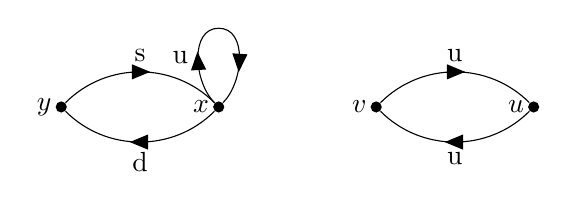
\begin{tikzpicture}
  \begin{feynman}
    % \node [inner sep=0.02cm](u) at (0,0) {\textbullet};
    % \node (v) at (2,0) {\textbullet};
    % \node (x) at (4,0) {\textbullet};
    % \node (y) at (6,0) {\textbullet};
    \node [inner sep=0.05cm, circle, fill](u) at (6,0) {};
    \node [inner sep=0.05cm, circle, fill](v) at (4,0) {};
    \node [inner sep=0.05cm, circle, fill](x) at (2,0) {};
    \node [inner sep=0.05cm, circle, fill](y) at (0,0) {};

    \draw (u) node[left] {$u$};
    \draw (v) node[left] {$v$};
    \draw (x) node[left] {$x$};
    \draw (y) node[left] {$y$};

    
    % \node[above = 1cm of u] (uu);
    \vertex[above = 1cm of u] (uu);
    \vertex[above = 1cm of v] (vv);
    \vertex[above = 1cm of x] (xx);
    \vertex[above = 1cm of y] (yy);
 % input nodes position and text
\diagram*{
  {[edges={fermion, quarter left}]
(v) --[edge label=u] (u),
(u) --[edge label=u] (v),
(y) --[edge label=s] (x),
(x) --[edge label=d] (y),
},

  {[edges={fermion}]
(x) -- [out=135, in=180, edge label=u] (xx) --[out=0, in=45] (x),
},
};
  \end{feynman}
\end{tikzpicture}

$-0.5556\ Tr[ \gamma_\mu L(u, v) \gamma_\nu L(v, u) ] Tr_s[ H(x, y) \gamma_5 L(y, x) \gamma_L ]_{c_3, c_2} Tr_s[ L(x, x) \gamma_L ]_{c_2, c_3} $


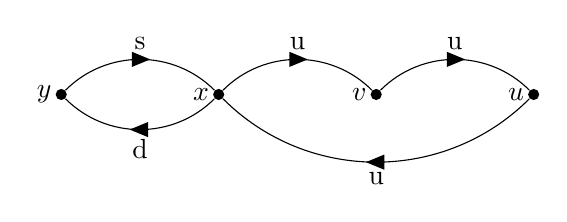
\begin{tikzpicture}
  \begin{feynman}
    % \node [inner sep=0.02cm](u) at (0,0) {\textbullet};
    % \node (v) at (2,0) {\textbullet};
    % \node (x) at (4,0) {\textbullet};
    % \node (y) at (6,0) {\textbullet};
    \node [inner sep=0.05cm, circle, fill](u) at (6,0) {};
    \node [inner sep=0.05cm, circle, fill](v) at (4,0) {};
    \node [inner sep=0.05cm, circle, fill](x) at (2,0) {};
    \node [inner sep=0.05cm, circle, fill](y) at (0,0) {};

    \draw (u) node[left] {$u$};
    \draw (v) node[left] {$v$};
    \draw (x) node[left] {$x$};
    \draw (y) node[left] {$y$};

    
    % \node[above = 1cm of u] (uu);
    \vertex[above = 1cm of u] (uu);
    \vertex[above = 1cm of v] (vv);
    \vertex[above = 1cm of x] (xx);
    \vertex[above = 1cm of y] (yy);
 % input nodes position and text
\diagram*{
  {[edges={fermion, quarter left}]
(u) --[edge label=u] (x),
(v) --[edge label=u] (u),
(x) --[edge label=u] (v),
(y) --[edge label=s] (x),
(x) --[edge label=d] (y),
},

  {[edges={fermion}]
},
};
  \end{feynman}
\end{tikzpicture}

$0.4444\ Tr_s[ L(x, u) \gamma_\mu L(u, v) \gamma_\nu L(v, x) \gamma_L ]_{c_2, c_3} Tr_s[ H(x, y) \gamma_5 L(y, x) \gamma_L ]_{c_3, c_2} $


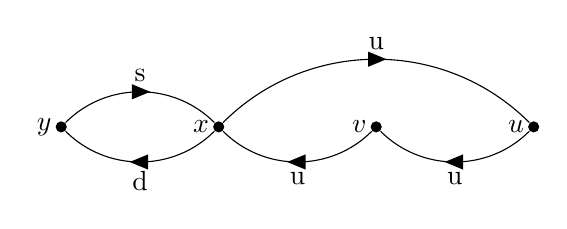
\begin{tikzpicture}
  \begin{feynman}
    % \node [inner sep=0.02cm](u) at (0,0) {\textbullet};
    % \node (v) at (2,0) {\textbullet};
    % \node (x) at (4,0) {\textbullet};
    % \node (y) at (6,0) {\textbullet};
    \node [inner sep=0.05cm, circle, fill](u) at (6,0) {};
    \node [inner sep=0.05cm, circle, fill](v) at (4,0) {};
    \node [inner sep=0.05cm, circle, fill](x) at (2,0) {};
    \node [inner sep=0.05cm, circle, fill](y) at (0,0) {};

    \draw (u) node[left] {$u$};
    \draw (v) node[left] {$v$};
    \draw (x) node[left] {$x$};
    \draw (y) node[left] {$y$};

    
    % \node[above = 1cm of u] (uu);
    \vertex[above = 1cm of u] (uu);
    \vertex[above = 1cm of v] (vv);
    \vertex[above = 1cm of x] (xx);
    \vertex[above = 1cm of y] (yy);
 % input nodes position and text
\diagram*{
  {[edges={fermion, quarter left}]
(v) --[edge label=u] (x),
(u) --[edge label=u] (v),
(x) --[edge label=u] (u),
(y) --[edge label=s] (x),
(x) --[edge label=d] (y),
},

  {[edges={fermion}]
},
};
  \end{feynman}
\end{tikzpicture}

$0.4444\ Tr_s[ L(x, v) \gamma_\nu L(v, u) \gamma_\mu L(u, x) \gamma_L ]_{c_2, c_3} Tr_s[ H(x, y) \gamma_5 L(y, x) \gamma_L ]_{c_3, c_2} $


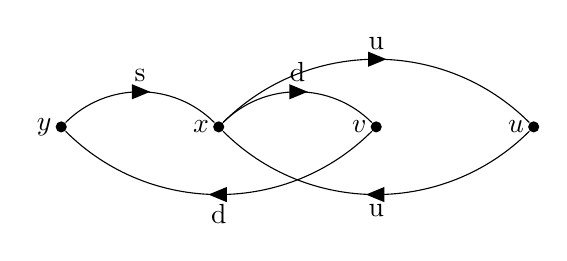
\begin{tikzpicture}
  \begin{feynman}
    % \node [inner sep=0.02cm](u) at (0,0) {\textbullet};
    % \node (v) at (2,0) {\textbullet};
    % \node (x) at (4,0) {\textbullet};
    % \node (y) at (6,0) {\textbullet};
    \node [inner sep=0.05cm, circle, fill](u) at (6,0) {};
    \node [inner sep=0.05cm, circle, fill](v) at (4,0) {};
    \node [inner sep=0.05cm, circle, fill](x) at (2,0) {};
    \node [inner sep=0.05cm, circle, fill](y) at (0,0) {};

    \draw (u) node[left] {$u$};
    \draw (v) node[left] {$v$};
    \draw (x) node[left] {$x$};
    \draw (y) node[left] {$y$};

    
    % \node[above = 1cm of u] (uu);
    \vertex[above = 1cm of u] (uu);
    \vertex[above = 1cm of v] (vv);
    \vertex[above = 1cm of x] (xx);
    \vertex[above = 1cm of y] (yy);
 % input nodes position and text
\diagram*{
  {[edges={fermion, quarter left}]
(u) --[edge label=u] (x),
(x) --[edge label=u] (u),
(y) --[edge label=s] (x),
(v) --[edge label=d] (y),
(x) --[edge label=d] (v),
},

  {[edges={fermion}]
},
};
  \end{feynman}
\end{tikzpicture}

$-0.2222\ Tr_s[ L(x, u) \gamma_\mu L(u, x) \gamma_L ]_{c_2, c_3} Tr_s[ H(x, y) \gamma_5 L(y, v) \gamma_\nu L(v, x) \gamma_L ]_{c_3, c_2} $


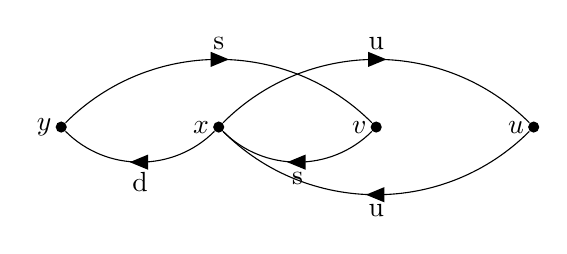
\begin{tikzpicture}
  \begin{feynman}
    % \node [inner sep=0.02cm](u) at (0,0) {\textbullet};
    % \node (v) at (2,0) {\textbullet};
    % \node (x) at (4,0) {\textbullet};
    % \node (y) at (6,0) {\textbullet};
    \node [inner sep=0.05cm, circle, fill](u) at (6,0) {};
    \node [inner sep=0.05cm, circle, fill](v) at (4,0) {};
    \node [inner sep=0.05cm, circle, fill](x) at (2,0) {};
    \node [inner sep=0.05cm, circle, fill](y) at (0,0) {};

    \draw (u) node[left] {$u$};
    \draw (v) node[left] {$v$};
    \draw (x) node[left] {$x$};
    \draw (y) node[left] {$y$};

    
    % \node[above = 1cm of u] (uu);
    \vertex[above = 1cm of u] (uu);
    \vertex[above = 1cm of v] (vv);
    \vertex[above = 1cm of x] (xx);
    \vertex[above = 1cm of y] (yy);
 % input nodes position and text
\diagram*{
  {[edges={fermion, quarter left}]
(u) --[edge label=u] (x),
(x) --[edge label=u] (u),
(v) --[edge label=s] (x),
(y) --[edge label=s] (v),
(x) --[edge label=d] (y),
},

  {[edges={fermion}]
},
};
  \end{feynman}
\end{tikzpicture}

$-0.2222\ Tr_s[ L(x, u) \gamma_\mu L(u, x) \gamma_L ]_{c_2, c_3} Tr_s[ H(x, v) \gamma_\nu H(v, y) \gamma_5 L(y, x) \gamma_L ]_{c_3, c_2} $


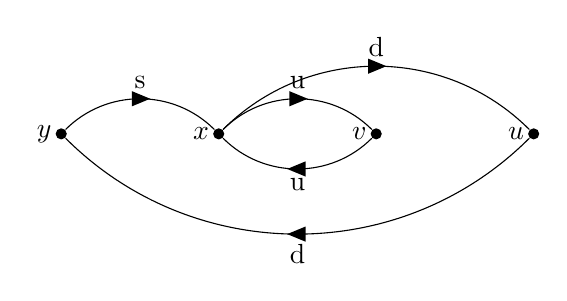
\begin{tikzpicture}
  \begin{feynman}
    % \node [inner sep=0.02cm](u) at (0,0) {\textbullet};
    % \node (v) at (2,0) {\textbullet};
    % \node (x) at (4,0) {\textbullet};
    % \node (y) at (6,0) {\textbullet};
    \node [inner sep=0.05cm, circle, fill](u) at (6,0) {};
    \node [inner sep=0.05cm, circle, fill](v) at (4,0) {};
    \node [inner sep=0.05cm, circle, fill](x) at (2,0) {};
    \node [inner sep=0.05cm, circle, fill](y) at (0,0) {};

    \draw (u) node[left] {$u$};
    \draw (v) node[left] {$v$};
    \draw (x) node[left] {$x$};
    \draw (y) node[left] {$y$};

    
    % \node[above = 1cm of u] (uu);
    \vertex[above = 1cm of u] (uu);
    \vertex[above = 1cm of v] (vv);
    \vertex[above = 1cm of x] (xx);
    \vertex[above = 1cm of y] (yy);
 % input nodes position and text
\diagram*{
  {[edges={fermion, quarter left}]
(y) --[edge label=s] (x),
(u) --[edge label=d] (y),
(x) --[edge label=d] (u),
(v) --[edge label=u] (x),
(x) --[edge label=u] (v),
},

  {[edges={fermion}]
},
};
  \end{feynman}
\end{tikzpicture}

$-0.2222\ Tr_s[ H(x, y) \gamma_5 L(y, u) \gamma_\mu L(u, x) \gamma_L ]_{c_3, c_2} Tr_s[ L(x, v) \gamma_\nu L(v, x) \gamma_L ]_{c_2, c_3} $


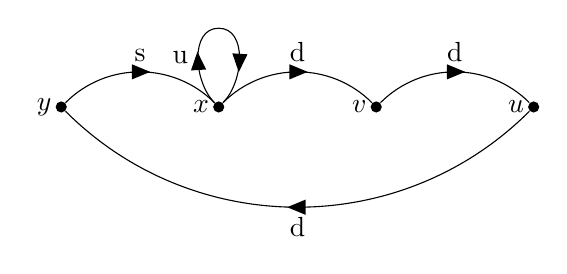
\begin{tikzpicture}
  \begin{feynman}
    % \node [inner sep=0.02cm](u) at (0,0) {\textbullet};
    % \node (v) at (2,0) {\textbullet};
    % \node (x) at (4,0) {\textbullet};
    % \node (y) at (6,0) {\textbullet};
    \node [inner sep=0.05cm, circle, fill](u) at (6,0) {};
    \node [inner sep=0.05cm, circle, fill](v) at (4,0) {};
    \node [inner sep=0.05cm, circle, fill](x) at (2,0) {};
    \node [inner sep=0.05cm, circle, fill](y) at (0,0) {};

    \draw (u) node[left] {$u$};
    \draw (v) node[left] {$v$};
    \draw (x) node[left] {$x$};
    \draw (y) node[left] {$y$};

    
    % \node[above = 1cm of u] (uu);
    \vertex[above = 1cm of u] (uu);
    \vertex[above = 1cm of v] (vv);
    \vertex[above = 1cm of x] (xx);
    \vertex[above = 1cm of y] (yy);
 % input nodes position and text
\diagram*{
  {[edges={fermion, quarter left}]
(y) --[edge label=s] (x),
(u) --[edge label=d] (y),
(v) --[edge label=d] (u),
(x) --[edge label=d] (v),
},

  {[edges={fermion}]
(x) -- [out=135, in=180, edge label=u] (xx) --[out=0, in=45] (x),
},
};
  \end{feynman}
\end{tikzpicture}

$0.1111\ Tr_s[ H(x, y) \gamma_5 L(y, u) \gamma_\mu L(u, v) \gamma_\nu L(v, x) \gamma_L ]_{c_3, c_2} Tr_s[ L(x, x) \gamma_L ]_{c_2, c_3} $


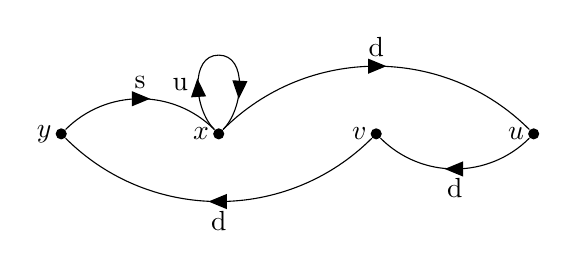
\begin{tikzpicture}
  \begin{feynman}
    % \node [inner sep=0.02cm](u) at (0,0) {\textbullet};
    % \node (v) at (2,0) {\textbullet};
    % \node (x) at (4,0) {\textbullet};
    % \node (y) at (6,0) {\textbullet};
    \node [inner sep=0.05cm, circle, fill](u) at (6,0) {};
    \node [inner sep=0.05cm, circle, fill](v) at (4,0) {};
    \node [inner sep=0.05cm, circle, fill](x) at (2,0) {};
    \node [inner sep=0.05cm, circle, fill](y) at (0,0) {};

    \draw (u) node[left] {$u$};
    \draw (v) node[left] {$v$};
    \draw (x) node[left] {$x$};
    \draw (y) node[left] {$y$};

    
    % \node[above = 1cm of u] (uu);
    \vertex[above = 1cm of u] (uu);
    \vertex[above = 1cm of v] (vv);
    \vertex[above = 1cm of x] (xx);
    \vertex[above = 1cm of y] (yy);
 % input nodes position and text
\diagram*{
  {[edges={fermion, quarter left}]
(y) --[edge label=s] (x),
(v) --[edge label=d] (y),
(u) --[edge label=d] (v),
(x) --[edge label=d] (u),
},

  {[edges={fermion}]
(x) -- [out=135, in=180, edge label=u] (xx) --[out=0, in=45] (x),
},
};
  \end{feynman}
\end{tikzpicture}

$0.1111\ Tr_s[ H(x, y) \gamma_5 L(y, v) \gamma_\nu L(v, u) \gamma_\mu L(u, x) \gamma_L ]_{c_3, c_2} Tr_s[ L(x, x) \gamma_L ]_{c_2, c_3} $


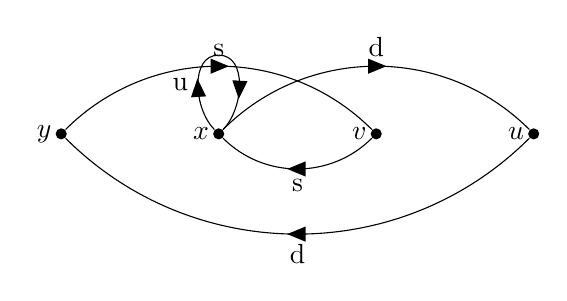
\begin{tikzpicture}
  \begin{feynman}
    % \node [inner sep=0.02cm](u) at (0,0) {\textbullet};
    % \node (v) at (2,0) {\textbullet};
    % \node (x) at (4,0) {\textbullet};
    % \node (y) at (6,0) {\textbullet};
    \node [inner sep=0.05cm, circle, fill](u) at (6,0) {};
    \node [inner sep=0.05cm, circle, fill](v) at (4,0) {};
    \node [inner sep=0.05cm, circle, fill](x) at (2,0) {};
    \node [inner sep=0.05cm, circle, fill](y) at (0,0) {};

    \draw (u) node[left] {$u$};
    \draw (v) node[left] {$v$};
    \draw (x) node[left] {$x$};
    \draw (y) node[left] {$y$};

    
    % \node[above = 1cm of u] (uu);
    \vertex[above = 1cm of u] (uu);
    \vertex[above = 1cm of v] (vv);
    \vertex[above = 1cm of x] (xx);
    \vertex[above = 1cm of y] (yy);
 % input nodes position and text
\diagram*{
  {[edges={fermion, quarter left}]
(v) --[edge label=s] (x),
(y) --[edge label=s] (v),
(u) --[edge label=d] (y),
(x) --[edge label=d] (u),
},

  {[edges={fermion}]
(x) -- [out=135, in=180, edge label=u] (xx) --[out=0, in=45] (x),
},
};
  \end{feynman}
\end{tikzpicture}

$0.1111\ Tr_s[ H(x, v) \gamma_\nu H(v, y) \gamma_5 L(y, u) \gamma_\mu L(u, x) \gamma_L ]_{c_3, c_2} Tr_s[ L(x, x) \gamma_L ]_{c_2, c_3} $


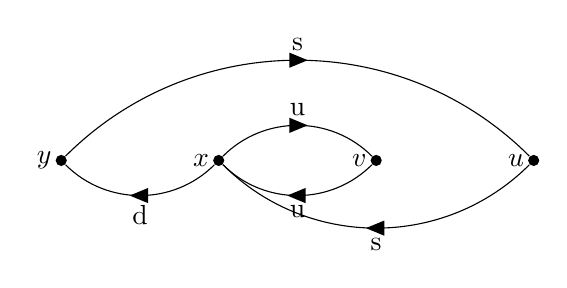
\begin{tikzpicture}
  \begin{feynman}
    % \node [inner sep=0.02cm](u) at (0,0) {\textbullet};
    % \node (v) at (2,0) {\textbullet};
    % \node (x) at (4,0) {\textbullet};
    % \node (y) at (6,0) {\textbullet};
    \node [inner sep=0.05cm, circle, fill](u) at (6,0) {};
    \node [inner sep=0.05cm, circle, fill](v) at (4,0) {};
    \node [inner sep=0.05cm, circle, fill](x) at (2,0) {};
    \node [inner sep=0.05cm, circle, fill](y) at (0,0) {};

    \draw (u) node[left] {$u$};
    \draw (v) node[left] {$v$};
    \draw (x) node[left] {$x$};
    \draw (y) node[left] {$y$};

    
    % \node[above = 1cm of u] (uu);
    \vertex[above = 1cm of u] (uu);
    \vertex[above = 1cm of v] (vv);
    \vertex[above = 1cm of x] (xx);
    \vertex[above = 1cm of y] (yy);
 % input nodes position and text
\diagram*{
  {[edges={fermion, quarter left}]
(u) --[edge label=s] (x),
(y) --[edge label=s] (u),
(x) --[edge label=d] (y),
(v) --[edge label=u] (x),
(x) --[edge label=u] (v),
},

  {[edges={fermion}]
},
};
  \end{feynman}
\end{tikzpicture}

$-0.2222\ Tr_s[ H(x, u) \gamma_\mu H(u, y) \gamma_5 L(y, x) \gamma_L ]_{c_3, c_2} Tr_s[ L(x, v) \gamma_\nu L(v, x) \gamma_L ]_{c_2, c_3} $


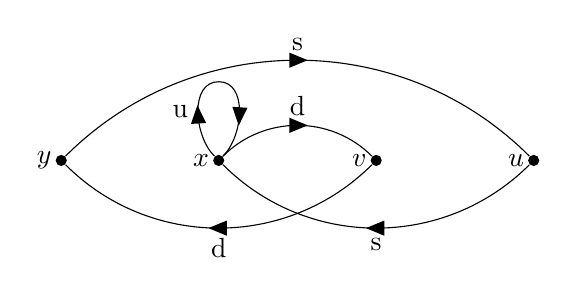
\begin{tikzpicture}
  \begin{feynman}
    % \node [inner sep=0.02cm](u) at (0,0) {\textbullet};
    % \node (v) at (2,0) {\textbullet};
    % \node (x) at (4,0) {\textbullet};
    % \node (y) at (6,0) {\textbullet};
    \node [inner sep=0.05cm, circle, fill](u) at (6,0) {};
    \node [inner sep=0.05cm, circle, fill](v) at (4,0) {};
    \node [inner sep=0.05cm, circle, fill](x) at (2,0) {};
    \node [inner sep=0.05cm, circle, fill](y) at (0,0) {};

    \draw (u) node[left] {$u$};
    \draw (v) node[left] {$v$};
    \draw (x) node[left] {$x$};
    \draw (y) node[left] {$y$};

    
    % \node[above = 1cm of u] (uu);
    \vertex[above = 1cm of u] (uu);
    \vertex[above = 1cm of v] (vv);
    \vertex[above = 1cm of x] (xx);
    \vertex[above = 1cm of y] (yy);
 % input nodes position and text
\diagram*{
  {[edges={fermion, quarter left}]
(u) --[edge label=s] (x),
(y) --[edge label=s] (u),
(v) --[edge label=d] (y),
(x) --[edge label=d] (v),
},

  {[edges={fermion}]
(x) -- [out=135, in=180, edge label=u] (xx) --[out=0, in=45] (x),
},
};
  \end{feynman}
\end{tikzpicture}

$0.1111\ Tr_s[ H(x, u) \gamma_\mu H(u, y) \gamma_5 L(y, v) \gamma_\nu L(v, x) \gamma_L ]_{c_3, c_2} Tr_s[ L(x, x) \gamma_L ]_{c_2, c_3} $


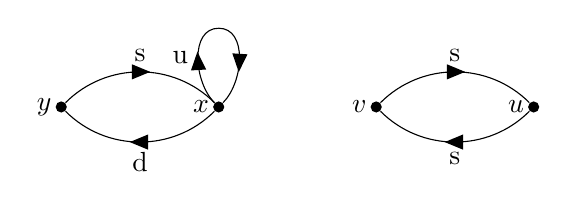
\begin{tikzpicture}
  \begin{feynman}
    % \node [inner sep=0.02cm](u) at (0,0) {\textbullet};
    % \node (v) at (2,0) {\textbullet};
    % \node (x) at (4,0) {\textbullet};
    % \node (y) at (6,0) {\textbullet};
    \node [inner sep=0.05cm, circle, fill](u) at (6,0) {};
    \node [inner sep=0.05cm, circle, fill](v) at (4,0) {};
    \node [inner sep=0.05cm, circle, fill](x) at (2,0) {};
    \node [inner sep=0.05cm, circle, fill](y) at (0,0) {};

    \draw (u) node[left] {$u$};
    \draw (v) node[left] {$v$};
    \draw (x) node[left] {$x$};
    \draw (y) node[left] {$y$};

    
    % \node[above = 1cm of u] (uu);
    \vertex[above = 1cm of u] (uu);
    \vertex[above = 1cm of v] (vv);
    \vertex[above = 1cm of x] (xx);
    \vertex[above = 1cm of y] (yy);
 % input nodes position and text
\diagram*{
  {[edges={fermion, quarter left}]
(v) --[edge label=s] (u),
(u) --[edge label=s] (v),
(y) --[edge label=s] (x),
(x) --[edge label=d] (y),
},

  {[edges={fermion}]
(x) -- [out=135, in=180, edge label=u] (xx) --[out=0, in=45] (x),
},
};
  \end{feynman}
\end{tikzpicture}

$-0.1111\ Tr[ \gamma_\mu H(u, v) \gamma_\nu H(v, u) ] Tr_s[ H(x, y) \gamma_5 L(y, x) \gamma_L ]_{c_3, c_2} Tr_s[ L(x, x) \gamma_L ]_{c_2, c_3} $


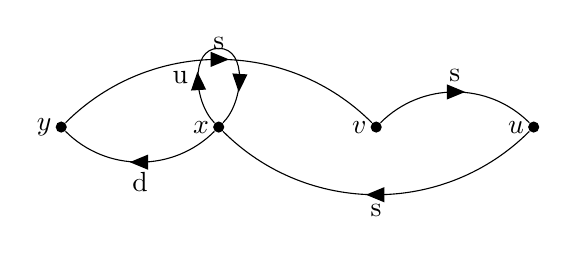
\begin{tikzpicture}
  \begin{feynman}
    % \node [inner sep=0.02cm](u) at (0,0) {\textbullet};
    % \node (v) at (2,0) {\textbullet};
    % \node (x) at (4,0) {\textbullet};
    % \node (y) at (6,0) {\textbullet};
    \node [inner sep=0.05cm, circle, fill](u) at (6,0) {};
    \node [inner sep=0.05cm, circle, fill](v) at (4,0) {};
    \node [inner sep=0.05cm, circle, fill](x) at (2,0) {};
    \node [inner sep=0.05cm, circle, fill](y) at (0,0) {};

    \draw (u) node[left] {$u$};
    \draw (v) node[left] {$v$};
    \draw (x) node[left] {$x$};
    \draw (y) node[left] {$y$};

    
    % \node[above = 1cm of u] (uu);
    \vertex[above = 1cm of u] (uu);
    \vertex[above = 1cm of v] (vv);
    \vertex[above = 1cm of x] (xx);
    \vertex[above = 1cm of y] (yy);
 % input nodes position and text
\diagram*{
  {[edges={fermion, quarter left}]
(u) --[edge label=s] (x),
(v) --[edge label=s] (u),
(y) --[edge label=s] (v),
(x) --[edge label=d] (y),
},

  {[edges={fermion}]
(x) -- [out=135, in=180, edge label=u] (xx) --[out=0, in=45] (x),
},
};
  \end{feynman}
\end{tikzpicture}

$0.1111\ Tr_s[ H(x, u) \gamma_\mu H(u, v) \gamma_\nu H(v, y) \gamma_5 L(y, x) \gamma_L ]_{c_3, c_2} Tr_s[ L(x, x) \gamma_L ]_{c_2, c_3} $


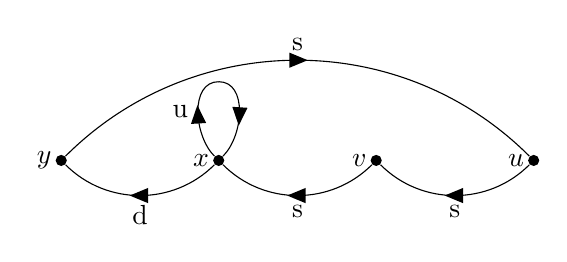
\begin{tikzpicture}
  \begin{feynman}
    % \node [inner sep=0.02cm](u) at (0,0) {\textbullet};
    % \node (v) at (2,0) {\textbullet};
    % \node (x) at (4,0) {\textbullet};
    % \node (y) at (6,0) {\textbullet};
    \node [inner sep=0.05cm, circle, fill](u) at (6,0) {};
    \node [inner sep=0.05cm, circle, fill](v) at (4,0) {};
    \node [inner sep=0.05cm, circle, fill](x) at (2,0) {};
    \node [inner sep=0.05cm, circle, fill](y) at (0,0) {};

    \draw (u) node[left] {$u$};
    \draw (v) node[left] {$v$};
    \draw (x) node[left] {$x$};
    \draw (y) node[left] {$y$};

    
    % \node[above = 1cm of u] (uu);
    \vertex[above = 1cm of u] (uu);
    \vertex[above = 1cm of v] (vv);
    \vertex[above = 1cm of x] (xx);
    \vertex[above = 1cm of y] (yy);
 % input nodes position and text
\diagram*{
  {[edges={fermion, quarter left}]
(v) --[edge label=s] (x),
(u) --[edge label=s] (v),
(y) --[edge label=s] (u),
(x) --[edge label=d] (y),
},

  {[edges={fermion}]
(x) -- [out=135, in=180, edge label=u] (xx) --[out=0, in=45] (x),
},
};
  \end{feynman}
\end{tikzpicture}

$0.1111\ Tr_s[ H(x, v) \gamma_\nu H(v, u) \gamma_\mu H(u, y) \gamma_5 L(y, x) \gamma_L ]_{c_3, c_2} Tr_s[ L(x, x) \gamma_L ]_{c_2, c_3} $




\end{document}